\section{System Architecture}
In this section the following main question is answered: 
\begin{quotation}
    \textit{''What would a system architecture look like to fulfill the described problem domain?''}
\end{quotation}
This includes the coverage of use cases, non-functional requirements, technologies used and how the tool will be designed.

\subsection{Use Cases}
A visual representation of the use cases with a use case diagram was deliberately omitted, because there is only one actor involved - the security advisor. The actor is not specifically mentioned in the use cases every time, because it is always the same.

\subsubsection{UC01 - Read Resultant Set of Policies}\label{UC01}
\begin{tcolorbox}
    \paragraph{Description} \ \\
    The specified audit policies are read and saved in a temporary file.
    \ \\
    \paragraph{Precondition} \ \\
    The system is running and the tool must possess administrator permissions.
    \ \\
    \paragraph{Main Success Scenario} 
    \begin{enumerate}
        \item Read the specified audit policies from the system
        \item Save the needed information from the audit policies in a temporary file for analysis purposes.
    \end{enumerate}   
\end{tcolorbox}

\subsubsection{UC02 - Analyse Audit Policies}\label{UC02}
\begin{tcolorbox}
    \paragraph{Description} \ \\
    The list which was created in UC01 is compared to a ''perfect settings''-list. Missing or wrong settings are going to be exported into a separate file.
    \ \\
    \paragraph{Precondition} \ \\
    UC01 is fulfilled: the temporary file is available.
    \ \\
    \paragraph{Main Success Scenario} 
    \begin{enumerate}
        \item The temporary files can be read
        \item Creates a list of incorrect settings
    \end{enumerate}   
\end{tcolorbox}
\subsubsection{UC03 - Find Event Logs}\label{UC03}
\begin{tcolorbox}
    \paragraph{Description} \ \\
    Event logs are search by ID and marked in an external file as found or missing.
    \ \\
    \paragraph{Precondition} \ \\
    The system is running and must have valid event logs. The tool must possess administrator permissions.
    \ \\
    \paragraph{Main Success Scenario} 
    \begin{enumerate}
        \item Search for the specified event logs from the local system
        \item Save the result from the search in a temporary file for analysis purposes.
    \end{enumerate}
\end{tcolorbox}


\subsubsection{UC04 - Analyse Found Event Logs}\label{UC04}
\begin{tcolorbox}
    \paragraph{Description} \ \\
    The implemented logic analyses, by defined event ids, which events occurred or are missing and creates a list of events that did not occurred or are not logged yet.
    \ \\
    \paragraph{Precondition} \ \\
    UC03 is fulfilled: the temporary file is available.
    \ \\
    \paragraph{Main Success Scenario} 
    \begin{enumerate}
        \item The temporary file can be read
        \item The list with the defined event ids is available
        \item Create a list of events which occurred and which are missing
    \end{enumerate}   
\end{tcolorbox}

\subsubsection{UC05 - Display missing or wrong system configuration}\label{UC05}
\begin{tcolorbox}
    \paragraph{Description} \ \\
    Based on the list created in UC02 and UC04 the user gets an overview of missing configurations (the result) which would improve the readiness of the system for a good attack detection.
    \ \\
    \paragraph{Precondition} \ \\
    The lists from UC02 and UC04 are available.
    \ \\
    \paragraph{Main Success Scenario} 
    \begin{enumerate}
        \item Displays a visual output of missing or wrong system configurations
    \end{enumerate}   
\end{tcolorbox}

\subsubsection{UC06 - Save Result to specific path}\label{UC06}
\begin{tcolorbox}
    \paragraph{Description} \ \\
    The actor has the possibility to save the overview from UC05 to a file in a specific path defined by the actor himself. This file contains the result from UC05 in a descriptive way.
    \ \\
    \paragraph{Precondition} \ \\
    UC05 is fulfilled: the result, respectively the overview is available
    \ \\
    \paragraph{Main Success Scenario} 
    \begin{enumerate}
        \item A file is saved to a specific path with the result from UC05
        \item The path can be defined by the actor
    \end{enumerate}   
\end{tcolorbox}


\subsection{Non Functional Requirements}

\begin{table}[H]
    \centering
    \def\arraystretch{2}
    \begin{tabular}{| p{2.5cm} | p{13.5cm} |} \hline
        \textbf{NFR-No.} & \textbf{Description}  \\ \hline
        NRF01 & After using the Toolkit the system must remain in the status quo. More specifically the system shall not deliberately alter any existing entry in the event logs and registry. However, the tool may produce new event logs.\\ \hline
        NFR02 & The user shall not notice significant performance degradation from the system when using the Toolkit. \\ \hline
        NFR03 & The Toolkit must be portable with no installation procedure before use. \\ \hline
        NFR04 & The minimal target version of the system for the Toolkit to run must be Microsoft Windows 10 Professional or Microsoft Server 2016. \\ \hline
        NFR05 & The Toolkit runs in one go, but can also be executed in single steps with the possibility to skip single steps (pause/abort in case of performance problems) \\ \hline
    \end{tabular}
    \caption{Non Functional Requirements}
\end{table}

\clearpage

\subsection{Technologies}
\subsubsection{Chosen Technologies}
\paragraph{PowerShell \& Visual Studio Code} \ \\
The decision as to which technology to use, was made in favour of PowerShell. The reason why PowerShell was used, was that it is close to the Microsoft Operating System and that it has a large and detailed documentation at its disposal. \ \\
\ \\
The scripts are written in Visual Studio Code with the extension packet ''PowerShell''. Visual Studio code is preferred to PowerShell ISE because it only requires working in one IDE for implementation and documentation.

\paragraph{LaTeX \& Visual Studio Code}\ \\
The documentation is written with LaTeX in Visual Studio Code wit the LaTeX Workshop extension. The main reason for LaTex was that the developers are already familiar with it. Furthermore, LaTeX offers a very simple way for referencing sources. On the other hand, we made the experience that with LaTeX the formatting is more reliable than for example when Microsoft Word is used.

\paragraph{Azure Cloud}\ \\
The test environment is set up, as described in section \ref{sec:testenvironment} ''\nameref{sec:testenvironment}'', in the azure cloud. One server and two clients form a virtual network, this enables developers to access it from anywhere to any given time. A disadvantage is the changing public IP-addresses to access the VMs. In the end, the advantages outweigh the disadvantages.

\paragraph{GitHub}\ \\
GitHub is used as a version control tool for source code and documentation. GitHub has been elected because of its good reputation and the experience the developers already gained with.

\paragraph{Continuous Integration}\ \\
Continuous Integration (CI) for Powershell is unfortunately not very widespread as has been shown after some time of research. Fortunately the article ''Converting a PowerShell Project to use Azure DevOps Pipelines'' \cite{CI} by Daniel Scott-Raynsford was found, which describes in detail how a CI environment can be set up in Microsoft Azure DevOps. Due to the fact that Azure DevOps offers a very simple and clear handling, as well as supports all common operating systems (Linux, Windows and MacOS), it was decided to set up the CI environment in Azure DevOps. The structure and the important findings are described in the Continuous Integration manual.

\subsubsection{Rejected Technologies}

\paragraph{Python}\ \\
The decision to use PowerShell and maybe C\# for a GUI instead of Python was made because the developers do not have much experience with Python. Also PowerShell is closer to the Microsoft-OS. With Python there is no guarantee that the libraries which would be used are as powerful to solve the requirements.


\clearpage

\subsection{Tool Design}
This section describes the process of the toolkit and explain the individual steps in detail. As mentioned in the Use Cases, the actor of this toolkit will be a security advisor, who will execute the toolkit.

\begin{figure}[H]
    \centering
    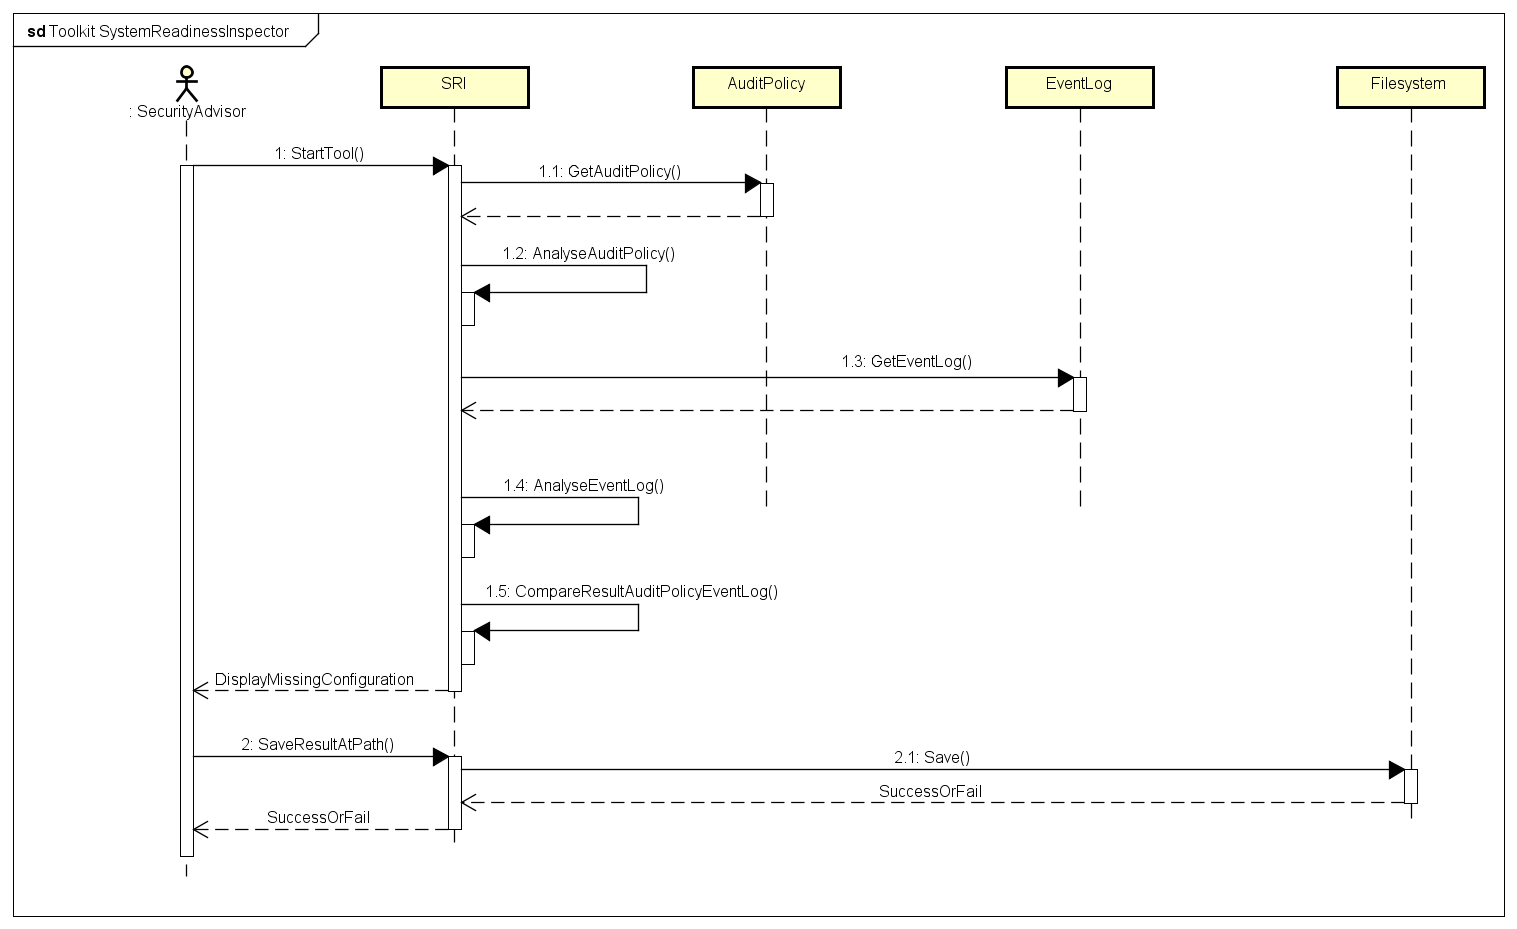
\includegraphics[width=0.8\linewidth]{assets/design-tool/SequenceDiagramSRI.png}
    \caption{Sequence Diagram SystemReadinessInspector - SRI}
\end{figure}

\subsubsection{GetAuditPolicy()}
This task is responsible to get all Audit Policies, which are relevant for logging the right events according to JPCERT/CCs study. To gather all information about the Audit Policies and the current state of its configuration  the ''Resultant Set of Policies'' (RSoP) must be read. \cite{RSoP} RSoP is a Microsoft snap-in to create a detailed report about the applied policy settings. 

\subsubsection{AnalyseAditPolicy()}
In this task the gathered information from the task GetAuditPolicy(), which is represented as a XML-File, is going to be analysed against the recommendation from JPCERT/CCs study (see \ref{JPCertStudy} \nameref{JPCertStudy}). the result of this analysis will be stored in a XML-based format in a temporary file.

\subsubsection{GetEventLog()}
This task is responsible for getting the event logs from the system. Therefor the command \lstinline|Get-EventLogs| \cite{Get-EventLogs} retrieves all logs from 'System', 'Application' and 'Security'. This logs are, to be analysed later, saved as a 'CSV' file to the current path were the PowerShell is running.

\subsubsection{AnalyseEvent()}
In this task the created 'CSV' file from GetEventLog() is used to analyse the collected logs. They are compared to a list provided by JPCERT to find out how ready the system would be if an enemy attack had taken place. The result of this comparison will be stored as a 'XML' file in order to visualise it.

